%! Author = mdh81
%! Date = 8/7/23

\documentclass{article}
\usepackage{amsmath}
\usepackage{mathtools}
\usepackage{graphicx}

\newcommand{\orthoMatrix}{
    \begin{bmatrix}
        \dfrac{2}{R-L} & 0 & 0 & -\dfrac{R+L}{R-L} \\ \\
        0 & \dfrac{2}{B-T} & 0 & -\dfrac{T+B}{T-B} \\ \\
        0 & 0 & \dfrac{2}{N-F} & -\dfrac{F+N}{N-F} \\ \\
        0 & 0 & 0 & 1
    \end{bmatrix}
}

\begin{document}
    \begin{center}
        \section*{Orthographic Projection Matrix}
    \end{center}

    \noindent In this document, we will derive the orthographic projection matrix created by this library.
    This matrix is for a right handed coordinate system and it follows OpenGL conventions for eye and clip space. \break
    \subsection*{OpenGL coordinate spaces}

    \subsubsection*{Eye coordinate space}
    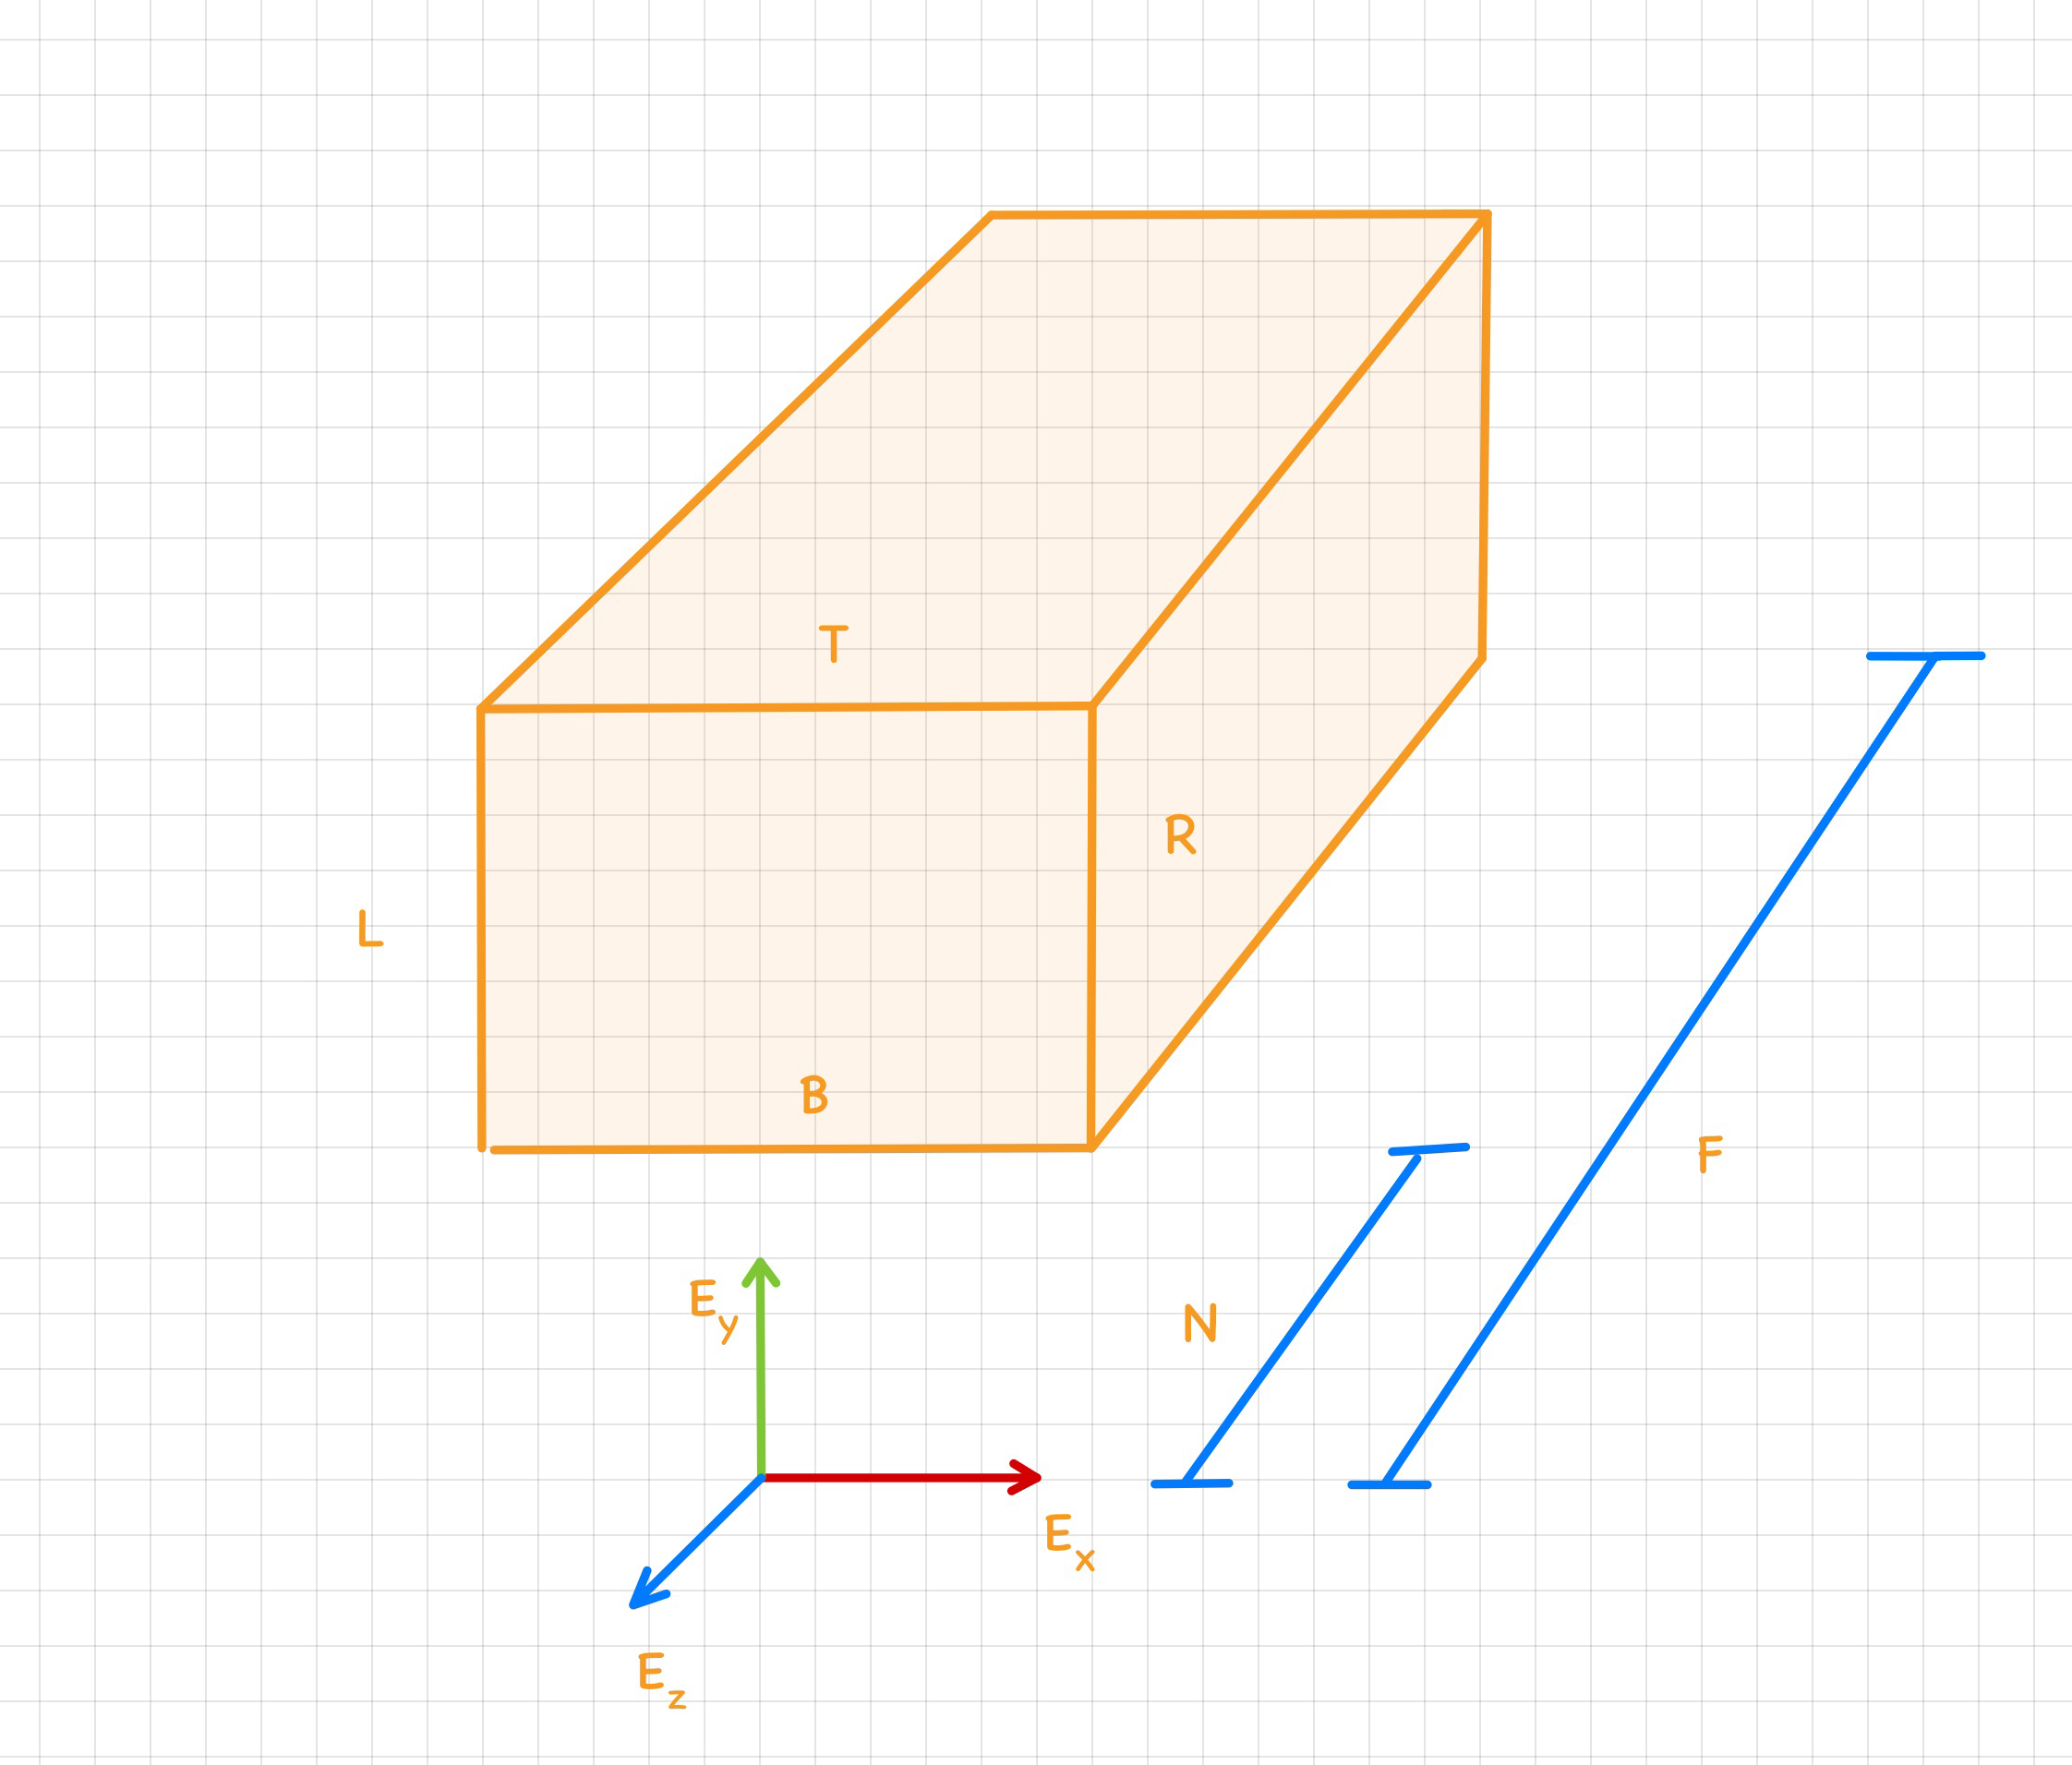
\includegraphics[width=0.75\textwidth]{../images/OrthoOpenGLEye.jpg}

    \noindent In the eye coordinate space, the eye or the camera is at the origin $[0,0,0]$ and it looks down the negative z-axis
    \subsubsection*{Normalized device coordinate space}
    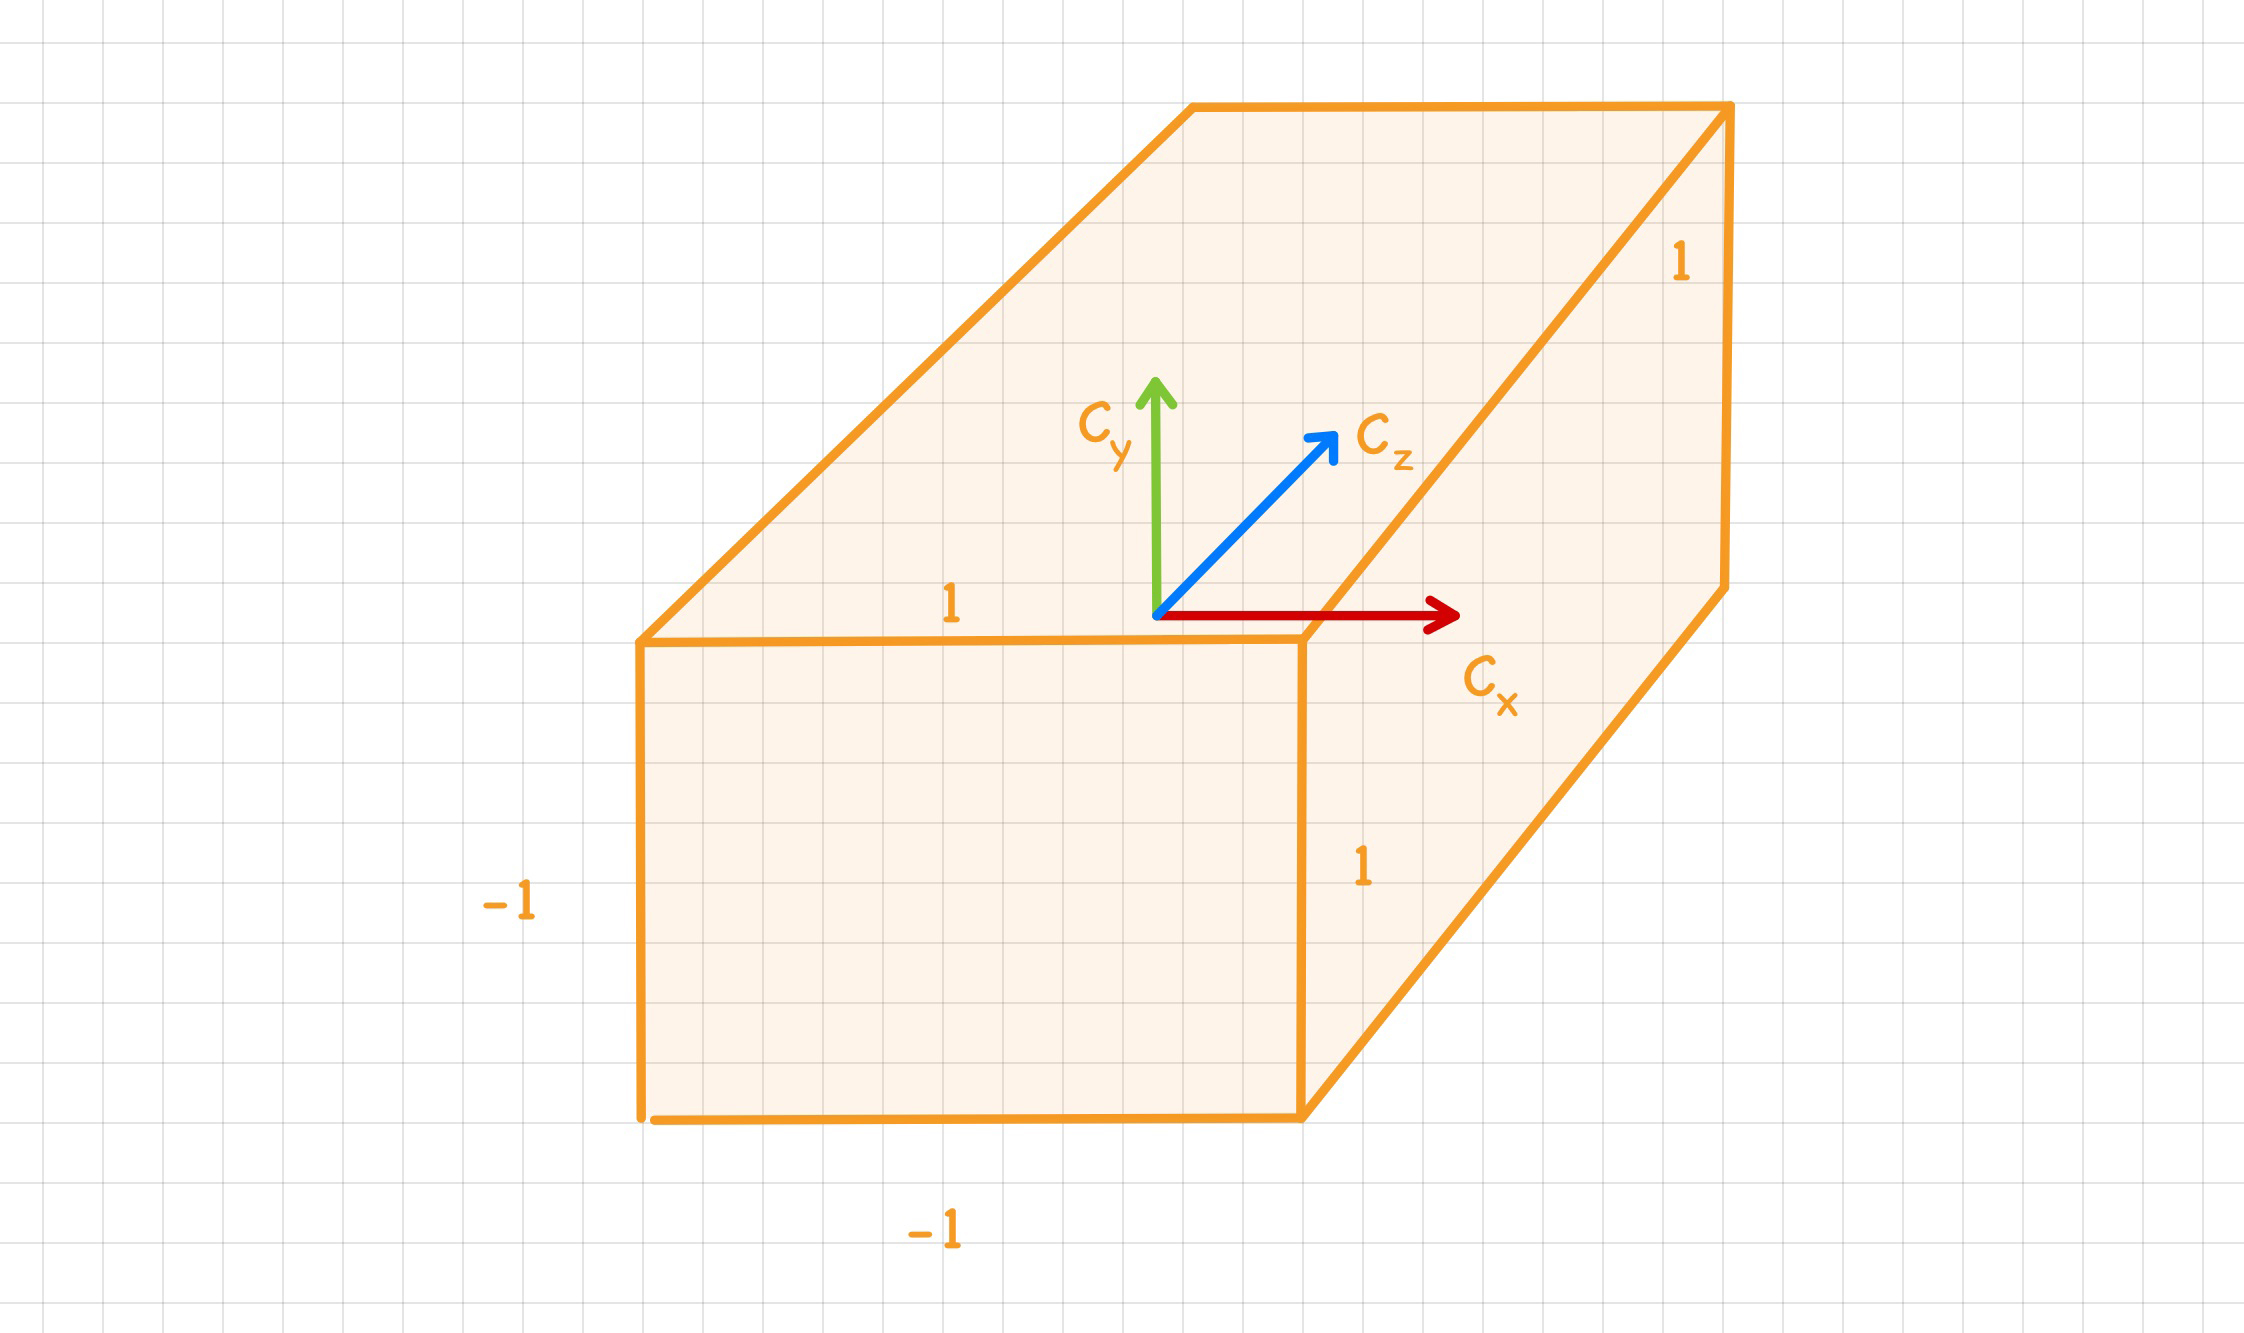
\includegraphics[width=0.75\textwidth]{../images/OrthoOpenGLClip.jpg}
    \paragraph \noindent In the normalized device coordinates space, the view volume is a cube of length 2. Coordinates of all points inside the view volume are in the range $[-1,1]$.\linebreak

    The key difference between the eye and clip space is the orientation of z-axis. In clip space, the positive z-axis is into the screen, in the eye space it is out of the screen.
    \footnote{I suspect the reason for $+z$ in clip space pointing into the screen is for ease of depth buffer comparison--if an incoming fragment's $z$ value is less than the previous depth value, it is accepted as it is nearer. If it was the other way around, larger z values would be considered closer to the camera and it sounds unnatural.} 
    \subsection*{Derivation for the orthographic matrix}
    \par \noindent The purpose of the orthographic matrix is to transform coordinates from the eye space to the clip space.

    \noindent In the eye space, a point's x-coordinate's relationship to the clipping planes is 
    
    \begin{align}
        L <= x <= R \label{eq:1} 
    \end{align}

    \noindent In the clip space, the same relationship is 
    
    \begin{align}
        -1 <= x <= 1
    \end{align}

    \noindent The goal of the orthographic matrix is to convert to the second form and it happens by the following set of operations

    \begin{align}
        \intertext{Subtract L from all sides of the inequality \ref{eq:1}}
        0 <= x-L <= R-L \\
        \intertext{Divide by R-L}
        0 <= \dfrac{x-L}{R-L} <= 1 \\
        \intertext{Multiply by 2}
        0 <= \dfrac{2(x-L)}{R-L} <= 2 \\
        \intertext{Subtract 1}
        -1 <= \dfrac{2(x-L)}{R-L} - 1 <= 1 \\
        \intertext{Simplifying}
        -1 <= \dfrac{(2x-2L-R+L)}{R-L} <= 1 \\
        -1 <= \dfrac{(2x-L-R)}{R-L} <= 1 \\
        -1 <= \dfrac{2x}{R-L}-\dfrac{R+L}{R-L} <= 1
    \end{align}

    \par\noindent Similarly for y, we can derive the relationship 
    
    \begin{align}
        -1 <= \dfrac{2y}{T-B}-\dfrac{T+B}{T-B} <= 1
    \end{align}

    \par\noindent For z, things get a little different because of the fact that both near and far clipping planes are planes are along the negative z-axis in the eye space. Since both near and far are negative, it must be observed that z-coordinate in eye space obey the relationship 
    
    \begin{align}
        F <= z <= N
    \end{align}

    \noindent Applying the same principle as above, we can continue the derivation

    \begin{align}
        \intertext{Subtract F from all sides of the inequality \ref{eq:1}}
        0 <= z-F <= N-F \\
        \intertext{Divide by N-F}
        0 <= \dfrac{z-F}{N-F} <= 1 \\
        \intertext{Multiply by 2}
        0 <= \dfrac{2(z-F)}{N-F} <= 2 \\
        \intertext{Subtract 1}
        -1 <= \dfrac{2(z-F)}{N-F} - 1 <= 1 \\
        \intertext{Simplifying}
        -1 <= \dfrac{(2z-2F-N+F)}{N-F} <= 1 \\
        -1 <= \dfrac{(2z-N-F)}{N-F} <= 1 \\
        -1 <= \dfrac{2z}{N-F}-\dfrac{F+N}{N-F} <= 1
    \end{align}

    \noindent Arranging these expressions in a matrix form such that $[x,y,z]$ will transform to these expressions produces matrix
    
    \begin{align}
        \orthoMatrix
    \end{align}

    \noindent Applying this matrix to $[x_{eye},y_{eye},z_{eye},1]$
    \begin{align}
        \orthoMatrix \times \begin{bmatrix} x_{eye} \\ \\ y_{eye} \\ \\ z_{eye} \\ \\ 1 \end{bmatrix}
    \end{align}

    \noindent produces the clip space coordinates \footnote{Note that the $w$ coordinate is $1$. Therefore, when this 4D coordinate is converted to 3D by dividing by $w$, the x and y coordinates remain unchanged. This is why there is no perspective foreshortening in orthographic projection}


    \begin{align}
        \begin{bmatrix} x_{clip} \\ \\ y_{clip} \\ \\ z_{clip} \\ \\ 1 \end{bmatrix} = 
        \begin{bmatrix} \dfrac{2x_{eye}}{R-L} - \dfrac{R+L}{R-L} \\ \\ \dfrac{2y_{eye}}{T-B} - \dfrac{T+B}{T-B} \\ \\ \dfrac{2z_{eye}}{N-F} - \dfrac{F+N}{N-F} \\ \\ 1 \end{bmatrix}
    \end{align}

    

    \noindent 
    
\end{document}
